\documentclass{homework}
\usepackage{homework}
\usepackage{pdfpages}

\title{COC473 - Lista 5}
\author{Pedro Maciel Xavier}
\register{116023847}
\notes{\textbf{Nota:} Na primeira seção da Lista estão os trechos de código dos programas pedidos. Na segunda parte, estão os resultados dos programas assim como a análise destes. Por fim, no apêndice está o código completo. Caso os gráficos estejam pequenos, você pode ampliar sem problemas pois foram renderizados diretamente no formato \texttt{.pdf}.}

\newcommand{\vecx}[3]{
	\ensuremath{\left[\begin{array}{@{}c@{}}
			#1\\
			#2\\
			#2
		\end{array}\right]}
}

\begin{document}
	
	\maketitle
	
	\section*{Programas}
	
	\questx[Integração Numérica]%%1
	
	A função \code{num\_int(f, a, b, n, kind)} calcula a integral $\int_{a}^{b} f(x) dx$ aproximada por $n$ pontos. O parâmetro nomeado opcional \code{kind} permite ao usuário escolher dentre as opções:
	\begin{itemize}[leftmargin=100pt]
		\item[\code{'polynomial'}] Integração Polinomial
		\item[\code{'gauss-legendre'}] Quadratura de \textit{Gauss-Legendre}
		\item[\code{'gauss-hermite'}] Quadratura de \textit{Gauss-Hermite}\footnote{Demanda condições especiais.}
		\item[\code{'romberg'}] Método de \textit{Romberg}
	\end{itemize}
	
	\lstinputlisting[firstline=649, lastline=677, style=fortranstyle, gobble=0]{../src/calclib.f95}
	
	\newpage
	
	\subquest[Integração Polinomial]%%2
	
	A Integração Polinomial foi implementada através da solução do sistema linear
	$${\displaystyle%%
			\begin{bmatrix}
				1 & 1  & \cdots & 1 \\
				x_1 & x_2 & \cdots & x_n \\
				\vdots & \vdots & \quad & \vdots \\
				x_{1}^{n-1} & x_{2}^{n-1} & \cdots & x_{n}^{n-1}
			\end{bmatrix}%%
			\begin{bmatrix}
				\omega_1\\
				\omega_2\\
				\vdots\\
				\omega_n
			\end{bmatrix} =%%
			\begin{bmatrix}
				b - a\\
				\frac{b^2 - a^2}{2}\\
				\vdots\\
				\frac{b^n - a^n}{n}\\
			\end{bmatrix}}$$
	onde os pesos de integração são dados pelas componentes $\omega_i$ da solução.
	
	\lstinputlisting[firstline=679, lastline=700, style=fortranstyle, gobble=0]{../src/calclib.f95}
	
	\subquest[Quadratura de \textit{Gauss-Legendre}]%%a
	
	A quadratura de \textit{Gauss-Legendre} foi calculada previamente para até $n = 128$ pontos através do sistema de computação algébrica da linguagem \textit{Mathematica}. O Código consta no apêndice.
	
	\lstinputlisting[firstline=702, lastline=725, style=fortranstyle, gobble=0]{../src/calclib.f95}
	
	\subquest[Quadratura de \textit{Gauss-Hermite}]%%a
	
	A quadratura de \textit{Gauss-Hermite} foi tabelada da mesma maneira que a anterior. Para utilizar este método, é preciso que a integração ocorra sobre todos os números reais, isto é, $[a, b] = [-\infty, \infty]$.
	
	\lstinputlisting[firstline=727, lastline=754, style=fortranstyle, gobble=0]{../src/calclib.f95}
	
	\newpage
	
	\subquest[Método de \textit{Romberg}]%%a
	
	Além dos métodos pedidos, implementei também a integração de \textit{Romberg} para conhecer mais esta técnica.
	
	\lstinputlisting[firstline=729, lastline=840, style=fortranstyle, gobble=0]{../src/calclib.f95}

	\subquest[Integração Adaptativa]%%4
	
	Implementei também a integração adaptativa, que permite calcular integrais dada uma tolerância. Assim, conseguimos resultados mais precisos para funções de comportamento irregular, isto é, aquelas que possuem derivadas com alto valor absoluto no intervalo de integração. Isso é feito subdividindo os trechos do intervalo $[a, b]$ de maneira que os subintervalos de maior irregularidade sejam analisados por mais pontos de integração. Esse método garante maior resolução sob demanda. \par
	
	Assim, foi possível obter valores mais precisos para fins de comparação.
	
	\lstinputlisting[firstline=756, lastline=790, style=fortranstyle, gobble=0]{../src/calclib.f95}
	
	\newpage
	\section*{Aplicações}
	
	\questx[Use o programa desenvolvido para obter o resultado numérico das seguintes integrais:]
	\begin{align*}
		I1 &= \int_{0}^{1} \frac{1}{\sqrt{2 \pi}} \exp \left(-\frac{x^2}{2}\right) dx\\
		I2 &= \int_{0}^{5} \frac{1}{\sqrt{2 \pi}} \exp \left(-\frac{x^2}{2}\right) dx
	\end{align*}

	Usando $n = 10$ pontos de integração:

	\lstinputlisting[firstline=1, lastline=16, style=blankstyle]{answer/L5.txt}
	
	\quest[Usando o seu programa e considerando $S_\sigma(\omega) = \text{RAO}(\omega)^2 S_\eta(\omega)$, onde%
	$$\text{RAO}(\omega) = \frac{1}{%%
	\sqrt{%%
		\left(1 - \left(\frac{\omega}{\omega_n}\right)^2\right)^2 + %%
		\left(2 \xi \frac{\omega}{\omega_n}\right)^2%%
		}%%
	}$$%%
	com $\omega_n = 1.0$ e $\xi = 0.05$ e $S_\eta(\omega) = 2.0$, obtenha $m_0$ e $m_2$ dados por:%%
		$$ m_0 = \int_{0}^{10} S_\sigma(\omega)~d\omega$$%%
		$$ m_2 = \int_{0}^{10} \omega^2 S_\sigma(\omega)~d\omega $$%%
	]
	
	\lstinputlisting[firstline=18, lastline=43, style=blankstyle]{answer/L5.txt}
	
	Com $n = 10$ pontos de integração, nenhum dos métodos se aproximou de fato do valor de referência. Para um estudo mais aprofundado, elaborei gráficos com os valores de cada método, considerando de 1 até 128 pontos de integração. Vejamos a figura:
	
	\begin{fig}
		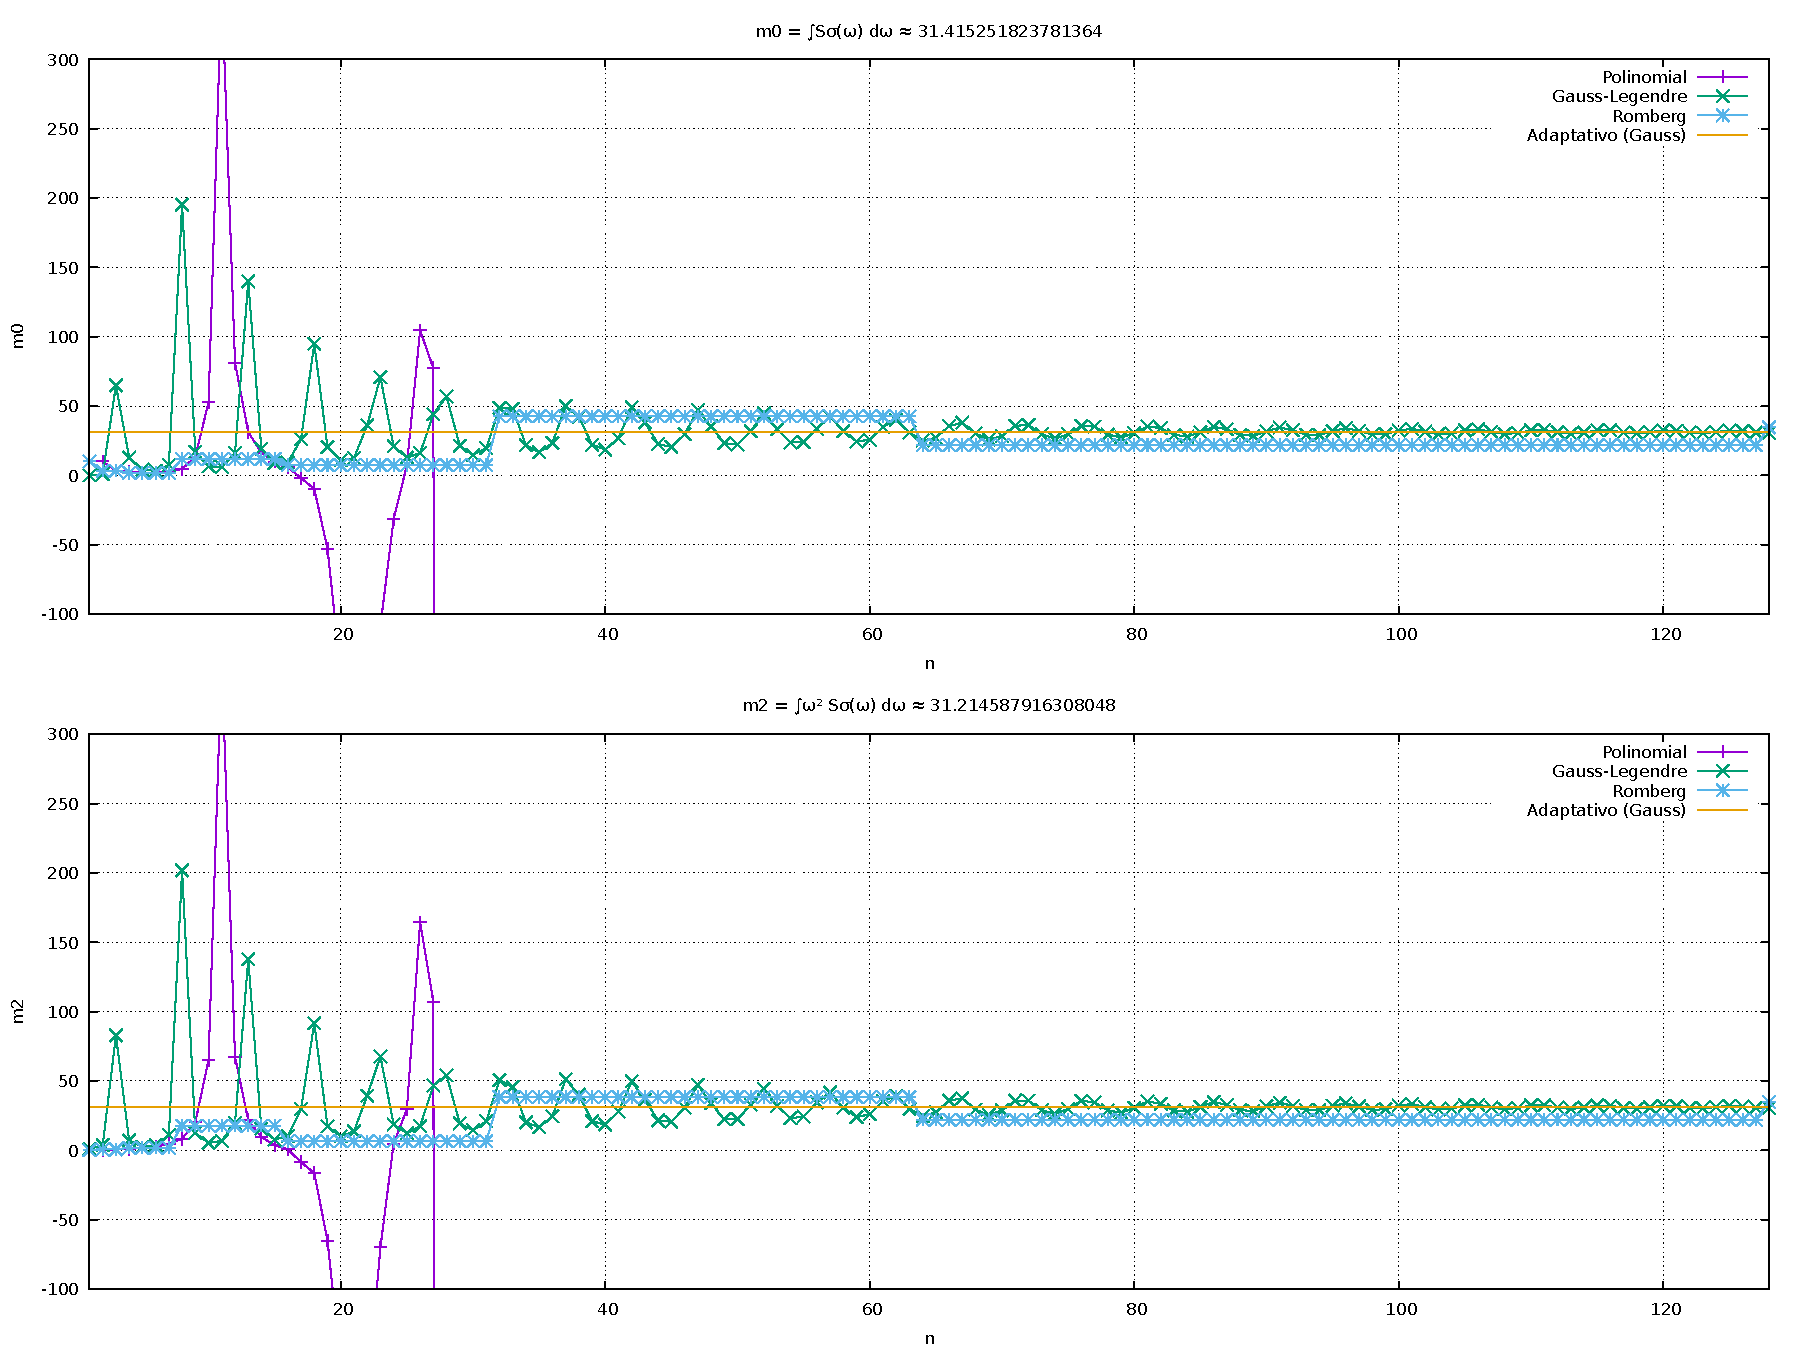
\includegraphics[width=\textwidth]{../src/plot/L5-Q3.pdf}
	\end{fig}
	
	O que vemos neste gráfico é, primeiramente, que a Integração Polinomial diverge completamente conforme aumentamos o número de pontos. A Quadratura de \textit{Gauss-Legendre} demonstra comportamento oscilatório ao redor da solução, apresentando valores próximos ao valor de referência com menos de 20 pontos de integração. Este resultando, contudo, ainda não é consistente e pequenas perturbações nas condições poderiam levar a erros catastróficos. Os valores passam a ser confiáveis quando se utiliza mais de 100 pontos de integração.\par
	%%
	O método de \textit{Romberg} possui uma certa sutileza. Iniciar o algoritmo com $n$ pontos de entrada faz com que este avalie a função em $2^n$ pontos. Por isso, para comparação com os algoritmos, são utilizados $\log_2(n)$ pontos como entrada. Isso faz com que se utilize $n$ pontos no total somente quando $n$ é potência de 2. Apesar disso, vemos que o método apresenta comportamento similar ao da quadratura, acompanhando a "amplitude" da oscilação.
	
	\questx[Repita o exercício anterior considerando \\$S_\eta(\omega) = {\displaystyle \frac{4 \pi^3 Hs^2}{\omega^5 Tz^4}} \exp\left(\displaystyle -\frac{16 \pi^3}{\omega^4 Tz^4}\right)$ com $Hs = 3.0$ e $Tz = 5.0$]
	
	\lstinputlisting[firstline=45, lastline=70, style=blankstyle]{answer/L5.txt}
	
	\begin{fig}
		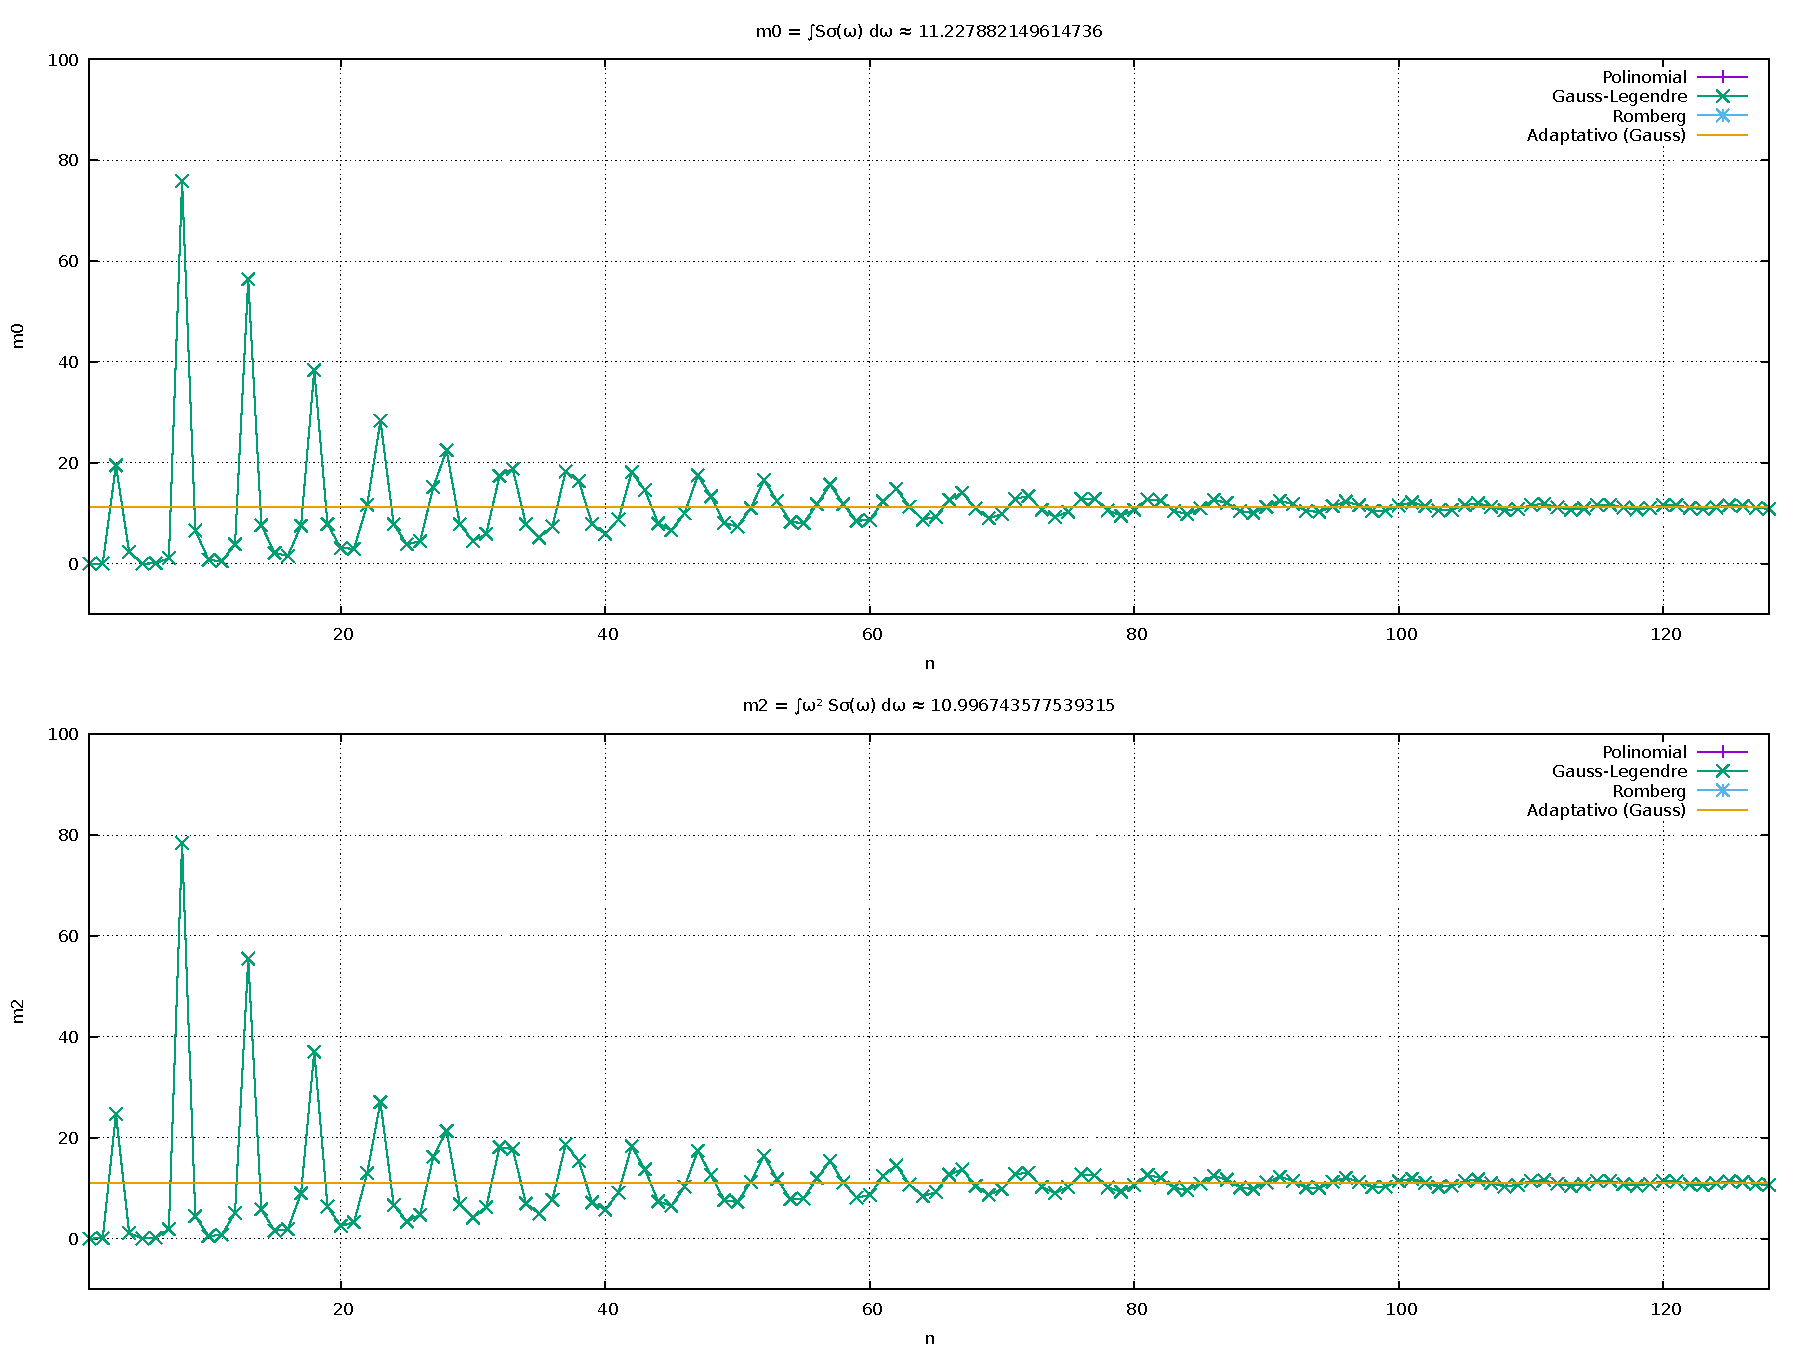
\includegraphics[width=\textwidth]{../src/plot/L5-Q4.pdf}
	\end{fig}
	
	A Quadratura de \textit{Gauss-Legendre} se mostrou oscilatória ao redor da solução como na questão anterior. Os métodos de Integração Polinomial e de \textit{Romberg}, no entanto, divergiram e rapidamente apresentaram valores inválidos (\code{NaN}) em seu resultado. O método de \textit{Romberg} é construído sobre a regra do trapézio e, portanto, apesar de ser um método adaptativo, está sujeito as mesmas vulnerabilidades.
	
	\quest[Com o programa desenvolvido, use o número mínimo de pontos de integração para integrar exatamente a integral abaixo pelos métodos da Integração Polinomial e da Quadratura de \textit{Gauss}.%%
	$$f(x) = 2 + 2x - x^2 + 3x^3$$%%
	$$\displaystyle A = \int_{0}^{4} f(x)~dx$$]%%

	Como o polinômio $f(x)$ tem grau 3, precisamos de $n = 4$ pontos para uma Integração Polinomial e $n = 2$ pontos para obter o valor exato pela Quadratura de \textit{Gauss}.

	\lstinputlisting[firstline=72, lastline=79, style=blankstyle]{answer/L5.txt}
	
	De fato, analiticamente temos%%
	$$A = \int_{0}^{4} 2 + 2x - x^2 + 3x^3~dx = \left[2x + x^2 - \frac{x^3}{3} + \frac{3x^4}{4}\right]_0^4 = \frac{584}{3} = 194.\overline{6}$$
	
	\quest[Use os valores da regra do Ponto médio e do Trapézio para estimar um valor mais aproximado para a integral abaixo. Obtenha também, a partir destes dois valores, qual seria o valor da integral caso tivesse sido usada a Regra de \textit{Simpson}. Resolva numericamente esta integral com o programa desenvolvido e compare os valores obtidos.]%% 6

	\subquest[Regra do Ponto médio]
	\begin{align*}
		A_\vec{M} \approx (b - a) \cdot f\left(\frac{b + a}{2}\right) &= 3 \cdot f\left(\frac{3}{2}\right)\\
		&= \displaystyle 3 \cdot \frac{1}{1 + \frac{9}{4}}\\
		&= \frac{12}{13} \approx 0.923
	\end{align*}
	
	\subquest[Regra do Trapézio]
	\begin{align*}
		A_\vec{T} \approx (b - a) \cdot \frac{f(a) + f(b)}{2} &= 3 \cdot \frac{f(0) + f(3)}{2}\\
		&= \displaystyle 3 \cdot \frac{\frac{1}{1 + 0} + \frac{1}{1 + 9}}{2}\\
		&= \frac{3}{2} \cdot \frac{11}{10} = \frac{33}{20} = 1.65
	\end{align*}
	
	\subquest[Regra de \textit{Simpson}]
	$$A_\vec{S} \approx \frac{2}{3} \cdot A_\vec{M} + \frac{1}{3} \cdot A_\vec{T} = \frac{2}{3} \cdot \frac{12}{13} + \frac{1}{3} \cdot \frac{33}{20} = \frac{303}{260} \approx 1.16538$$
	
	Calculando numericamente com $n = 10$ pontos de integração:
	\lstinputlisting[firstline=82, lastline=89, style=blankstyle]{answer/L5.txt}
	O erro relativo é de aproximadamente $\displaystyle \frac{|1.249 - 1.165|}{|1.249|} \approx 6.71\%$

	\quest[A quadratura de \textit{Gauss} conforme apresentada em aula é usada para integrais com limites de integração conhecidos e é também chamada de Quadratura de \textit{Gauss-Legendre}. Para integrais com um ou ambos limites de integração envolvendo $-\infty$ ou $\infty$ usa-se a quadratura \textit{Gauss-Hermite}. Pesquise sobre esta técnica e desenvolva uma rotina (similar ao Exercício 1) para resolver as seguintes integrais:%
	$$A_1 = \int_{-\infty}^{1} \frac{1}{\sqrt{2 \pi}} \exp \left(-\frac{x^2}{2}\right)~dx$$%%
	$$A_2 = \int_{-\infty}^{+\infty} \frac{x^2}{\sqrt{2 \pi}} \exp \left(-\frac{x^2}{2}\right)~dx$$%%
	]
	
	A quadratura de \textit{Gauss-Hermite} se aplica a integrais na forma
		$$ \int_{-\infty }^{+\infty } K(x) f(x)~dx $$
	onde dizemos que $K(x) = e^{-x^{2}}$ é o núcleo da integral. Mesmo que a função que desejamos integrar não esteja sendo multiplicada por este termo, podemos sempre utilizar a propriedade fundamental da exponenciação $e^{a} \cdot e^{b} = e^{a + b}$ para separar a função deste núcleo. Dizemos que $1 = e^{0} = e^{x^2 - x^2} = e^{x^2} \cdot e^{-x^2}$ e assim construímos a função $\tilde{f}(x) = f(x) \cdot e^{x^2}$. Com isso concluímos que
	$$\int_{-\infty}^{+\infty}f(x)~dx = \int_{-\infty}^{+\infty} K(x) \tilde{f}(x)~dx$$

	\subquest[$A_1$]\\
	No cálculo de $A_1$ vamos separar a integral em duas partes, fatorando as constantes:
	\begin{align*}
		A_1 &= \int_{-\infty}^{1} \frac{1}{\sqrt{2 \pi}} \exp \left(-\frac{x^2}{2}\right)~dx\\[1ex]
		&= \frac{1}{\sqrt{2 \pi}} \left[ \int_{-\infty}^{0} \exp \left(-\frac{x^2}{2}\right)~dx + \int_{0}^{1} \exp \left(-\frac{x^2}{2}\right)~dx \right] \\[1ex]
	\end{align*}
	Em seguida, multiplicamos o primeiro termo por $e^{x^2} \cdot e^{-x^2} = 1$, o que não altera o valor da integral:
	\begin{align*}
		A_1 &= \frac{1}{\sqrt{2 \pi}} \left[ \int_{-\infty}^{0} e^{-x^2} \cdot e^{x^2} \cdot \exp \left(-\frac{x^2}{2}\right)~dx + \int_{0}^{1} \exp \left(-\frac{x^2}{2}\right)~dx \right] \\[1ex]
		&= \frac{1}{\sqrt{2 \pi}} \left[ \int_{-\infty}^{0} e^{-x^2} \cdot \exp \left(\frac{x^2}{2}\right)~dx + \int_{0}^{1} \exp \left(-\frac{x^2}{2}\right)~dx \right] \\[1ex]
	\end{align*}
	Por fim, usamos o fato de que ambas as integrais atuam sobre funções pares para usar a seguinte relação:
	$$f(x) = f(-x)~~\forall x \implies \int_{-L}^{0} f(x)~dx = \frac{1}{2} \int_{-L}^{+L} f(x)~dx ~~\forall L \ge 0$$
	Portanto,
	\begin{align*}
		A_1 &= \frac{1}{\sqrt{8 \pi}} \left[ \int_{-\infty}^{+\infty} e^{-x^2} \cdot \exp \left(\frac{x^2}{2}\right)~dx + \int_{-1}^{1} \exp \left(-\frac{x^2}{2}\right)~dx \right] \\[1ex]
	\end{align*}
	Agora estamos prontos para calcular a integral do primeiro termo pela quadratura de \textit{Gauss-Hermite} com $f(x) = \exp \left(x^2 / 2\right)$ assim como a integral do segundo termo pela quadratura de \textit{Gauss-Legendre} com $f(x) = \exp \left(-x^2 / 2 \right)$. No fim, dividimos o resultado por $\sqrt{8 \pi}$.
	
	\subquest[$A_2$]\\
	A integral $A_2$, por sua vez, se encontra mais próxima da forma que se espera para aplicar a quadratura de \textit{Gauss-Hermite}. Multiplicando a integral pelo produto de exponenciais como fizemos anteriormente obtemos:
	\begin{align*}
		A_2 &= \int_{-\infty}^{+\infty} e^{-x^2} \cdot \frac{x^2}{\sqrt{2 \pi}} \cdot e^{x^2} \cdot \exp \left(-\frac{x^2}{2}\right)~dx \\[1ex]
		&= \int_{-\infty}^{+\infty} e^{-x^2} \cdot \frac{x^2}{\sqrt{2 \pi}} \cdot \exp \left(\frac{x^2}{2}\right)~dx
	\end{align*}
	Portanto, basta integrar $\displaystyle f(x) = \frac{x^2}{\sqrt{2 \pi}} \cdot \exp \left(\frac{x^2}{2}\right)$ segundo a quadratura de \textit{Gauss-Hermite}.\par
	%%
	Com $n = 10$ pontos de integração obtive os seguintes resultados:
	
	\lstinputlisting[firstline=91, lastline=100, style=blankstyle]{answer/L5.txt}
	
	\setcounter{quests}{0}
	
	\newpage
	
	\section*{Complemento - Derivadas Numéricas}
	
	\questx[{Escreva um programa que permita o cálculo numérico da derivada de uma função num ponto $x$ pelas regras de diferenças finitas:%%
	\begin{enumerate}[label=\alph*)]%%
		\item Diferença central
		\item Passo à frente
		\item Passo atrás
	\end{enumerate}~
	}]

	\lstinputlisting[firstline=15, lastline=52, style=fortranstyle]{../src/calclib.f95}

	\questx[Automatize no programa anterior o procedimento de extrapolação de Richard ($p = 1$ ou $p = 2$, a ser escolhido pelo usuário) para melhorar a estimativa da derivada de uma função $f(x)$ num ponto $x$ qualquer.]
	
	\lstinputlisting[firstline=842, lastline=880, style=fortranstyle]{../src/calclib.f95}
	
	\questx[Utilizando os programas desenvolvidos nas Tarefas 1 e 2, calcule as derivadas das seguintes funções nos pontos indicados e compare com os valores analíticos.%%
	\begin{enumerate}%%
		\item $\displaystyle f(x) = x^3 + e^{-x};~~ x = 3;$
		\item $\displaystyle f(x) = x^{1/3} + \log(x);~~ x = 2;$
		\item $\displaystyle f(x) = 1 - \exp\left(- x^2 / 25\right);~~ x = 6;$
	\end{enumerate}~
	]%%
	Nos resultados vemos os valores aproximados por cada modalidade de derivada, seguidos pelo erro $|\delta y|$, calculado em relação ao valor da derivada analítica.\par
	
	%%
	\lstinputlisting[firstline=105, lastline=214, style=blankstyle]{answer/L5.txt}

	\pagebreak
	\appendixpage
	\appendix \section*{Código - Programa Principal}
	\lstinputlisting[style=fortranstyle, gobble=0]{../src/main5.f95}
	\appendix \section*{Código - Definição das Funções}
	\lstinputlisting[style=fortranstyle, gobble=0]{../src/funcmod.f95}
	\appendix \section*{Código - Métodos Numéricos}
	\lstinputlisting[style=fortranstyle, gobble=0]{../src/calclib.f95}
	\appendix \section*{Código - Métodos com Matrizes}
	\lstinputlisting[style=fortranstyle, gobble=0]{../src/matrixlib.f95}
	\appendix \section*{Código - Biblioteca Auxiliar}
	\lstinputlisting[style=fortranstyle, gobble=0]{../src/utillib.f95}
	\appendix \section*{Código - Biblioteca de Plotagem}
	\lstinputlisting[style=fortranstyle, gobble=0]{../src/plotlib.f95}
	\appendix \section*{Código - Quadraturas pelo \textit{Mathematica}}
	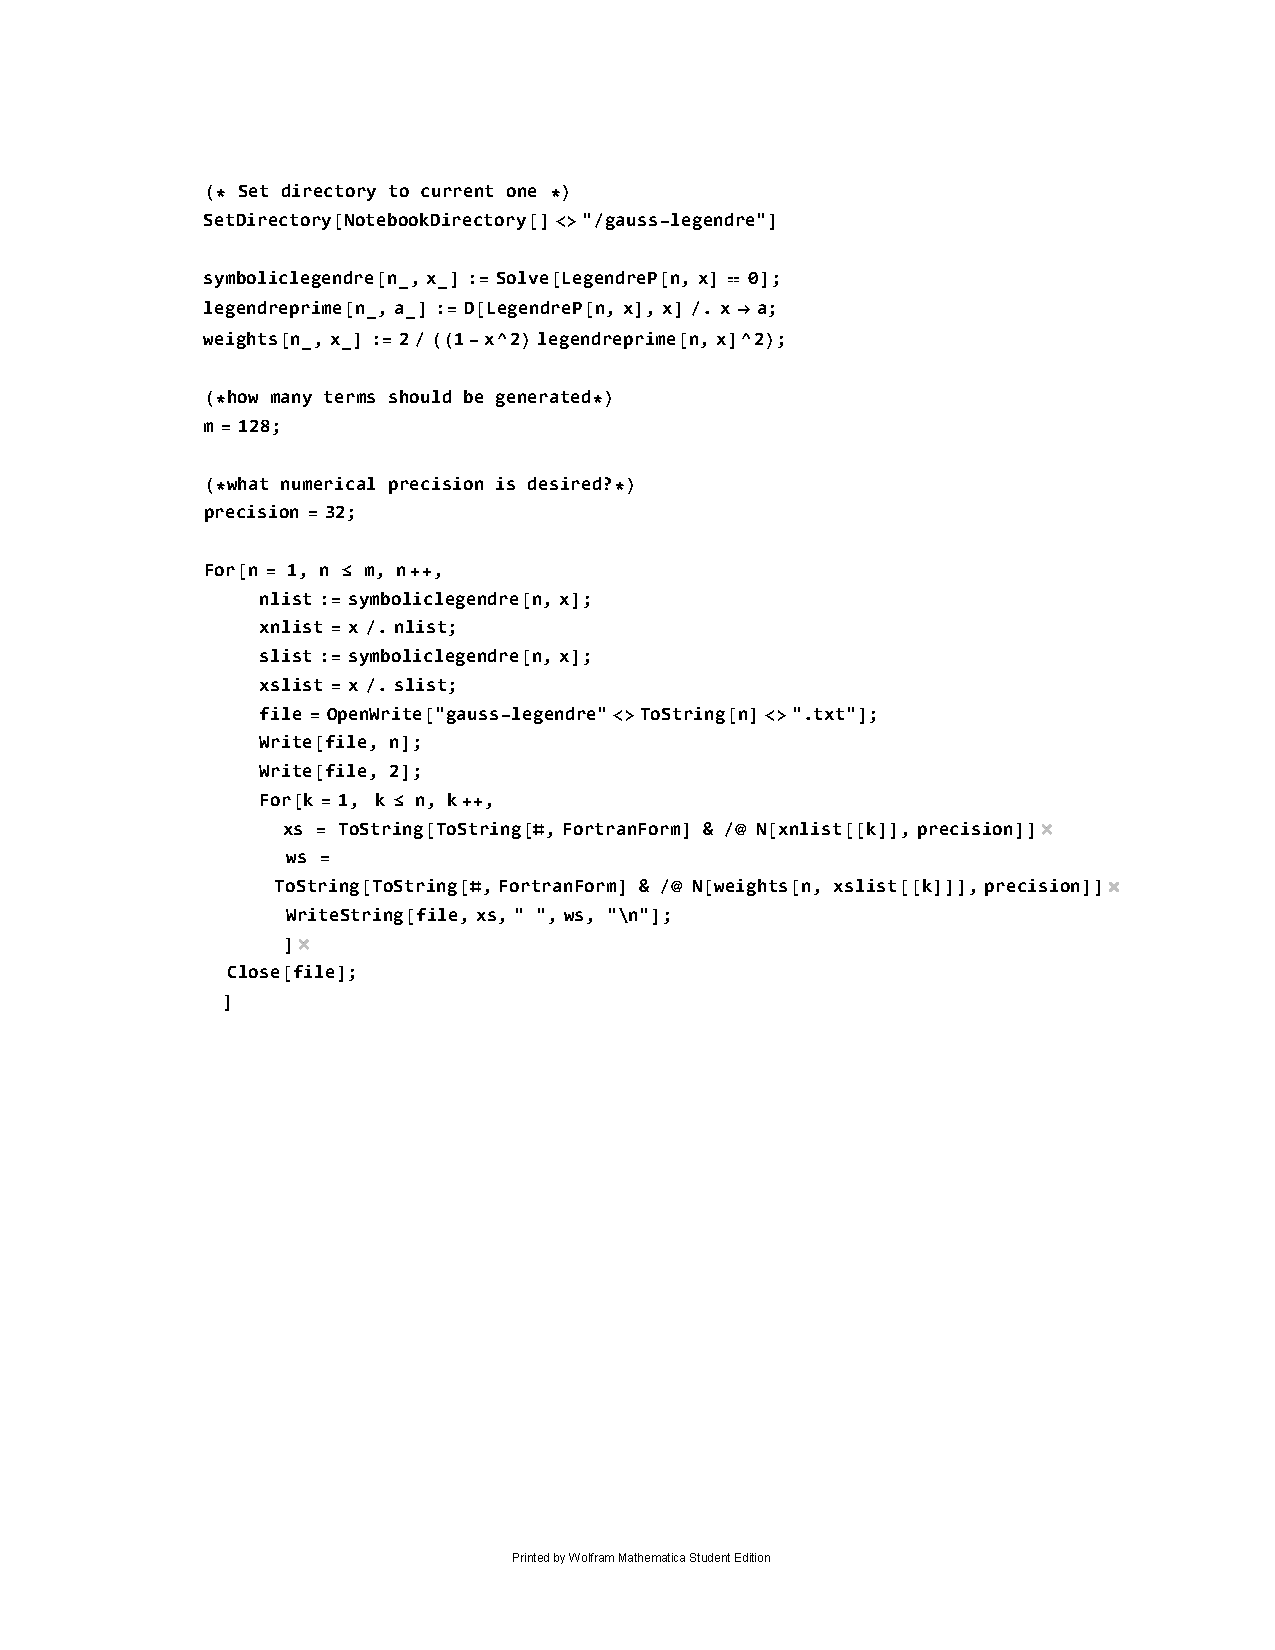
\includepdf[pages=-]{../src/quadratures/quadrature.pdf}
%	\begin{thebibliography}{10}
%		
%	\end{thebibliography}
\end{document}
